\documentclass[11pt]{article}

\usepackage{graphicx}
\usepackage{amsmath}
\numberwithin{figure}{section}
\numberwithin{table}{section}
\usepackage{sidecap}
\usepackage{geometry}

\usepackage{acl2015}
\usepackage{times}
\usepackage{url}
\usepackage{latexsym}

\usepackage{fancyref}
\usepackage{subcaption}

\usepackage[font={small}]{caption}

%\setlength\titlebox{5cm}

% You can expand the titlebox if you need extra space
% to show all the authors. Please do not make the titlebox
% smaller than 5cm (the original size); we will check this
% in the camera-ready version and ask you to change it back.


\title{Recipe Completion Using Machine Learning Techniques}

\author{Lingzhen Chen \\
  Department of Information Engineering And Computer Science \\
  Università degli Studi di Trento\\
  {\tt lingzhen.chen@studenti.unitn.it}
\\}

\date{2016-07-22}

\begin{document}
\maketitle
\begin{abstract}
  In recent years, recipe related collaborative knowledge sharing platform have increasingly impacted the way individuals gain access to their cooking guidance. Moreover, there is a variety of available websites and applications providing recipe recommendation services, which are mainly achieved by content based recommender system that takes advantage of user preferences and profiles. The purpose of this paper is to develop an advanced recipe completion system in order to provide a solution in the scenario where a user is in possession of a numbers of ingredients, and needs a possible additional ingredient recommendation to complete a recipe. The process of representing ingredients by word embeddings are introduced, as well as how we incorporate their contextualized features from recipes. Several models are proposed and tested.  
  %The process for  recipe completion task are discussed in the paper, several models with different configurations are proposed incorporating contextualized features from recipe and ingredient data as word embedding vectors . 
  Models are evaluated on their ability to retrieve a missing ingredient in the test recipe and their performance are compared. Results reveal that the proposed models with proper configurations are able to perform well on the task.
\end{abstract}

\section{Introduction}

Recipe sharing websites and applications have freed people from the cumbersome process of searching printed recipes in a cookbook. 
 Especially in the past several decades, with a booming amount of recipe data being updated online through various platforms, and the development of sophisticated recommendation modelling approaches, it became ever-growingly feasible to incorporate abundant recipe data to provide a better recipe search or recommendation service.
 Not only did the recipe recommendation systems enriched the source which one obtains his or her cooking instructions, but also improved the efficiency of collaborative knowledge sharing.
 Tremendous endeavour has been put into design a more comprehensive computational model for feature representation of recipes or ingredients, as well as to develop a more robust recipe recommendation system.

Many existing recipe recommendation system are based on building user profiles, collecting information about their preferences and feedbacks in order to make prediction. It often requires user to know the name of a recipe in order to perform a search, or it would recommend a similar recipe to which a user had tried or liked.
 However, these recommendation systems are not solution in a very common scenario in life, that is, when a user already have some ingredients at hand, but does not know what he or her can do with them. 
 Thus, one may wonder if there is a possibility to do perform recommendation not by user profiles as we discussed, but by discovering the connections and relations among ingredients in recipes. 
 Assuming that a user has some ingredient available in his or her refrigerator without knowing what kind of dish these ingredients can form, an interesting solution to the problem would be a system that takes a list of ingredients as input, decide if there is a possibility that by adding one or more ingredients, they would make a reasonable recipe. To be able to perform such a prediction, the system needs to incorporate the information of an ingredient such as its food category, flavour components, or its occurrence time in the data set to generate a feature representation of the ingredient.
 % It is accomplished by using Word2Vec tool ~\cite{Mikolov:2013} to train vector representation of the ingredients. 
 It is also necessary to have a comprehensive template that represents a recipe by the ingredients that it contains. 
 Moreover, an optimization function is the key to solve the recipe recommendation task.
 This paper demonstrates the procedure and experiments of developing such recipe recommendation system. We discuss in detail the data set, the consideration and design of our model, the mathematical fundamentals, extensive experimental results and a throughout evaluation of the performance.

The rest of the paper is organized as follows. Section 2 explores the related work. Section 3 analyses the data set that is used and introduces the pre-processing steps that is carried out. Section 4 illustrates a detailed description of the model, followed by the presentation of implementation and experiment results in Section 5 and Section 6. Last but not the least, final conclusions are drawn in Section 7.

\section{Related Work}

Recipe recommendation has been a subject of may prior work. 
Typically, system developers have tried to perform recipe recommendation based on user profiles, such as their ratings on recipes in the past ~\cite{Forbes:2011} or their browsing history ~\cite{Ueda:2011}. The algorithm is designed to find similar recipe based on the ingredients in common, either treating each ingredient equally ~\cite{Freyne:2010} or identifying major ingredient ~\cite{Zhang:2008}. 
~\cite{Wang:2008} tried to represent recipes as graphs that are based on ingredients and cooking instructions. ~\cite{Teng:2012} also tried to construct ingredient network incorporating the likelihood of ingredients to co-occur, as well as the potential of one ingredient to act as a substitute for another.
~\cite{Clercq:2016} employed machine learning methods, to be more specific, non-negative matrix factorization method and two-step regularized least squares method to perform recipe completion task. ~\cite{Forbes:2011} also implemented a content-boosted matrix factorization algorithm which incorporates content information directly as a linear constraint.
Our solutions aim to solve a problem that is similar to which they intended to tackle by non-negative matrix factorization method in ~\cite{Clercq:2016}.


\section{Dataset}

The dataset used in this report consists of two files, recipes.csv and ingredients.csv, which are both taken from ~\cite{Ahn:2011}. The recipe file contains 56,498 recipes originating from 11 different cuisines. For each recipe, the geographical category and ingredient are listed. In the recipe file, there are in total 381 different ingredients, which forms the ingredient file together with their food category.

\subsection{Data Preprocessing}

Before using the dataset, some pre-precessing on the data are done in order to filter out  uncommon examples in the dataset, as well as to obtain more unbiased results in later experiments. For starters, the geographical information, i.e. the first column in the recipe file is removed. And the recipes with less than 3 ingredients are deleted from the recipe file. The new file (\textit{recipe\_as\_input.txt}), which will be the input for training embeddings of ingredients, consists of 55,001 entries. This modification does not change the fact that there are 381 different ingredients appear in the recipe file. However in order to increase the confidence of trained vector. Ingredients with occurrence less than 75 times are removed from the ingredient file. The new ingredient file (\textit{ingredients\_major.txt}), consists of 248 unique entries of ingredients. These ingredients still covers 52,375 recipes (more than 95\% percent of the original recipe file). In later sections where the experiment settings are introduced, it would be clear that this occurrence restriction is also applied while calculating vector representations, by specifying the parameter $min-count$ (minimum occurrence of the ingredient in training file ) as 75.

With these two files, we are able to generate matrices that represents the relationships between recipes and ingredients. A binary matrix $M$ is calculated with shape $(m \times n)$, where $m$ indicates the number of recipes and $n$ indicates the number of ingredients. This matrix serves as an one-hot encoding of data to show which ingredients a recipe contains. The index in the matrix preserves the order recipes and ingredients appear in the data files. And its transpose, $M^T$ is also useful when the information about which recipes that an ingredients appears in is needed. These two matrices are saved as \textit{reci\_ingr\_matrix.txt} and \textit{ingr\_reci\_matrix.txt}. Moreover, we obtain the co-occurrence matrix by calculating $R = M^T \times M$ and the common ingredient matrix by calculating $C = M \times M^T$. They are both integer matrix where $R_{ij}$ indicates the number of times ingredient $i$ and ingredient $j$ occur together in one recipe, and $C_{ij}$ indicates the number of common ingredients that recipe $i$ and recipe $j$ have. These matrices are saved as \textit{co\_occur\_matrix.txt} and \textit{common\_ingr\_marix.txt}.
\subsection{Data Distribution}
In our data file, 248 ingredients comes from 13 different food categories, among which the category 'vegetable' covers 51 (20.6\%), while 'animal\_product' and 'plant' has the lowest coverage, with both only 4 ingredients.
The minimum number of ingredients in a a recipe is 3, while the maximum is 32. The average length of recipe is 8.

\section{Methodology}
\label{sec:Methodology}

In this experiment, we aim to develop an advanced recipe recommendation system that, according to an incomplete recipe input, can suggest one or more ingredient to complete it. The suggestion is computed by calculating the similarity scores between potential target ingredients and the incomplete input recipe (i.e. the recipe template).

In order to achieve this goal. There are couple issues that we need to tackle. Firstly, a suitable feature representation of ingredients and recipes data is needed. Secondly, a model for recovering the missing ingredient in the recipe needs to be developed. Last but not the least, a series of performance measures need to be decided for evaluating the feature representation quality and the model performance.

In this section, fundamentals about the model the mathematical principles behind the model are described in detail.

\subsection{Vector Representation}
\label{sec:Vector Representation}

For starters, in order to capture the characteristics of an ingredient, it is necessary to chose a suitable representation method for the ingredients in the data set. As discussed in previous sections, on the one hand, the characteristics of an ingredient are indicated by its own properties such as its total occurrence frequency in the data set and its similar ingredients. On the other hand, the characteristics are also manifested by its relationship with other ingredients, that is to say, whether an ingredient tends to co-occur often with some other ingredients or not.
In order to predict if one ingredient is potentially a fit for the input recipe template, the similarity between the context of a recipe template and the set of ingredients that the target ingredient often co-occur with plays an important role.

Thus in order to capture these features of an ingredient, we exploit the ability of the tool Word2Vec to generate distributed representation of words and phrase. The vector representation generated by this tool is called word embeddings, which is shown to carry semantic meanings and are very useful in various natural language processing tasks. As documented in the paper ~\cite{Mikolov:2013}, they introduced a task that given a word pair $(a,b)$ and a word $c$, the task aims to find a word $d$, such that the relation between $c$ and $d$ is similar to that between $a$ and $b$. Word2vec tool provides an efficient implementation of the continues bag-of-word(CBOW) and skip-gram architectures for computing vector representations of words. Intuitively, the vectors of similar ingredients would have shorter distance in the vector space, compared to the those that are not similar to each other. Hence the similar ingredient points would tend to cluster in the vector space. %How well the vectors are clustered together are later used as a metric to evaluate the quality of the vector representation generated.

There are a number of hyper-parameters that are needed to be decided for the training process. And for deciding which vector would be the best for our model, they are evaluated by maximizing average similarity metrics. These aspects are discussed in the later section of the paper.

\subsection{Similarity Measures}
\label{sec:Similarity Measures}

The similarity between ingredients plays a crucial role in predicting the fitness of a target ingredient to a recipe template. While using Word2Vec, the similarity can be calculated by the cosine distance of vectors. In addition, the contextual similarity of an ingredient is also taken into consideration by calculating raw and normalized similarity metric in terms of recipes they are in. 

\textit{\textbf{ Cosine Similarity and Angular Similarity}}

First and foremost, an intuitive way to compare the similarity between vectors are by comparing there distance in the vector space. There are a variety of distance metrics that we can choose from. In this paper, we use cosine distance due to its ability to capture the similarity in vectors regardless of the magnitude of the elements in the vectors.

For ingredient vector $A$ and $B$, their cosine similarity is calculated by formula
\begin{equation}
\begin{split}
cosine\_similarity(A,B) = \cos(\theta) = \\
\frac{A \cdot B}{\|A\|\|B\|} = \frac{\sum_{i=1}^{n}A_iB_i}{\sqrt{\sum_{i=1}^{n}A_i^2}\sqrt{\sum_{i=1}^{n}B_i^2}}
\end{split}
\end{equation}

where $n$ denotes the dimension of the vector.
It is worth mentioning that if the vectors contain negative values, then the cosine similarity is bounded between $[-1,1]$. 

In order to obtain a similarity metric that is bounded between [0,1], transformation needs to be made from cosine similarity to angular similarity by following formula
\begin{equation}
\begin{split}
	&angular\_similarity(A,B) = \\
	&1- \frac{\cos^{-1}(cosine\_similarity(A,B))}{\pi}
\end{split}
\end{equation}

where the $cosine\_similarity(A,B)$ is what defined by formula (1). In this case, the value 0 indicates absolute dissimilarity between vectors and 1 means two vectors are identical.

\textit{\textbf{ Raw Similarity and Normalized Similarity}}

This similarity measure is designed to capture the context information of an ingredient in terms of recipes that it is in. The binary recipe vector $I_R$ (248 x 1) is represented in one-hot encoding indicating which ingredients it contains. For ingredient $i$ and ingredient $j$, the sets of recipes contains them are represented by $I$ and $J$. The similarity between ingredient $i$ and ingredient $j$ is given by formula

\begin{equation}
sim(i,j) = \frac{1}{n_I}\frac{1}{n_J}\sum_{I_{R_i} \in I}\sum_{ I_{R_j} \in J} <I_{R_i},I_{R_j}>
\end{equation}

Intuitively, it is summing up the value of pair-wise dot product of the recipe that contains ingredient $i$ and the recipe that contains ingredient $j$ between all the pairs in $I$ and $J$. Then this value is divided by the scalar product of numbers of elements in $I$ and $J$ (i.e. the number of recipes contains ingredient $i$ multiply that contains ingredient $j$). It is the average number of common ingredients between ingredient $i$'s context (i.e. the recipes contain $i$) and ingredient $j$'s context.
The value of this similarity metric ranges from lower limit $0$, which means that the contextual recipes share no common ingredient, to the upper limit-- the maximum length of recipe, which means the contextual recipes are identical. 

It is obvious that the upper limit varies according to the length of recipes, which could introduce some biased interpretation of our observation.
Hence, in order to make it more evident and make the comparison between this similarity measure and other similarity measure easier, it is useful to normalize the result to obtain a score bounded in [0,1]. The normalized similarity measure is given by formula

\begin{equation}
sim(i,j) = \frac{\sum_{I_{R_i} \in I} \sum_{ I_{R_j} \in J} \frac{2 \cdot |I_{R_i} \cap I_{R_j}|}{|I_{R_i}| + |I_{R_j}|}}{|I| \cdot |J|}
\end{equation}

where a recipe contains ingredient $i$ is treated as a set of ingredients $I_{R_{i}}$ while that contains ingredient $j$ is represented by $I_{R_{j}}$. $|I_{R_{i}}|$ denotes the length of a recipe that contains ingredient $i$ and $|I|$ represents the number of all recipes that contains ingredient $i$.

\subsection{Optimization Model}
\label{sec:Optimization Model}

The next step would be to design a model that can predict if a target ingredient is a fit for the input recipe template. It is achieved by calculating the profit score of an ingredient with regard to the recipe template, the scores of all the candidate ingredients are ranked and the top $n$ ingredients with the highest scores are chosen.
The profit between the ingredient and recipe template can be calculated by formula:

\begin{equation}
\begin{split}
 \text{profit}(T, i) &= \frac{\sum_{j \in T \setminus \{ i \}} \text{cooccur}(i, j)}{|T \setminus \{ i \}|}\\
 					 &- \frac{\sum_{j, k \in T} \text{cooccur}(j, k)}{\binom{|T|}{2}} \\
 					&+ \frac{\max_{j \in T} \text{context}(i, j)}{2} \\
 					&+ \frac{\min_{j \in T} \text{context}(i, j)}{2}
\end{split}
\end{equation}

where $T$ is the template and $i$ is the target ingredient. The function cooccur($i,j$) is the co-occurrence score between two ingredients in the dataset, which is given by the normalized PMI (pairwise mutual information) that is calculated by formula

\begin{equation}
		\text{npmi}(x, y) = \frac{\text{pmi}(x,y)}{- \log p(x, y)}
\end{equation}

where

\begin{equation}
	\begin{split}
		\text{pmi}(x,y) &= \log \frac{p(x,y)}{p(x)p(y)} \\
			   &=\log p(x,y) - \log(p(x)p(y))
	\end{split}
\end{equation}
 
in which

\begin{equation}
	p(x) = \frac{N_{x}}{N}
\end{equation}
%\begin{equation}
%	p(x) = \frac{\text{\# of recipes containing } x}{\text{\# of recipes}}
%\end{equation}

%\begin{equation}
%	p(y) = \frac{\text{\# of recipes containing } y}{\text{\# of recipes}}
%\end{equation}

where $N_x$ is the number of recipes containing ingredient $i$ and $N$ is the total number of recipes. And

\begin{equation}
	p(x,y) = \frac{N_{xy}}{N}
\end{equation}

in which $N_{xy}$ is the number of recipes containing both ingredient $x$ and ingredient $y$.
%\begin{equation}
%	 p(x, y) = \frac{\text{\# of recipes containing } x \text{ and } y}{\text{\# of recipes}}
%\end{equation}

The value of npmi$(x,y)$ ranges in $[-1,1]$. Similar to the processing of similarity metrics described in the previews section, we make this value bounded within $[0,1]$ by adding one and dividing by 2, which gives us:

\begin{equation}
	 \text{npmi}_{0\!-\!1}(x, y) = \frac{\log (p(x) p(y))}{2 \log p(x, y)}
\end{equation}

In formula (5), the function context($i,j$) is the similarity function between ingredient that takes into account the context, which is calculated by formula (2) or formula (4), depending on which context information to be used.

\subsection{Evaluation Metrics}
\label{sec:Evaluation Metrics}

The model produces a list of predicted ingredients sorted by the profit score as output. Thus for evaluating the performance of our model, following 5 metrics can be used as a reference:

1) Mean position of the eliminated ingredient in the ordered list of suggested ingredients.

2) Median position of the eliminated ingredient in the ordered list of suggested ingredients:

3) Percentage of test recipes for which the eliminated ingredient is located in the top 10 of suggested ingredients.

4) Percentage of the eliminated ingredient being predicted at the first rank.

5) The mean AUC. The AUC is defined as the area under the ROC curve. Since there is only one positive observation, the AUC is directly related to the rank of the eliminated ingredient and can be computed as:


\begin{equation}
AUC = 1-(\frac{rank-1}{N^-}) = \frac{N^-+1-rank}{N^-}
\end{equation}

with $N^-$ the number of negative observations and rank the position of the eliminated ingredient in the ordered list of suggested ingredients.

\section{Implementation}
\label{sec:Implementation}

The implementation of the experiments follows the step described in the previous chapter. Firstly, the vectors of ingredients are trained with different sets of hyper-parameters. After analysing the vectors according to the average similarity score they have in formed clusters, the best vector representation is chosen for calculating contextual information of ingredients with regard to recipe. The contextual information will also be calculated according to the normalized similarity discussed in the previous chapter. Apart from the Word2Vec tool, the rest of the experiments are implemented in Python.

\subsection{Word2Vec Parameter Settings}
\label{sec:Word2Vec Parameter Settings}

First of all, experiments are done with fine-tuning the hyper-parameter of the vector training by Word2Vec. 
In order to find a optimal combination of hyper-parameters, coordinate descent method is used. It is a non-derivative optimization algorithm. Line search is done along one coordinate direction at current point in each iteration, and different coordinate directions are used cyclically through the procedure to find the local optimal of a function. In our experiment, it means optimizing one hyper-parameter at a time, until we find an optimal value. And then this hyper-parameter is set to its optimal value before we start to fine-tune the next one.
Some critical parameters are $size$, $negative$, $window$, $cbow$, $hs$, $sample$, and $min-count$.

$-cbow$ indicates if continues bag of word model (-cbow 1) or skip gram model (-cbow 0) is used; from literature, skip-gram model works better with low frequency words, but overall these two model should generate similar results.

$-hs$ indicates if hierarchical softmax is used or not.

$-size$ indicates the dimension of vector.

$-negative$ indicates the number of negative samples that is used during training

$-window$ indicates the context window size surrounding a word (i.e. ingredient) that is considered during training. This value is set to maximum of total ingredient number in recipe --32.

$-sample$ mainly affects the speed of training but not much the result.

$-min-count$ the minimum times a word occur in the data set for it to be considered in the vocabulary.

In addition, since the vectors need to be clustered for deciding the one with best quality, the number of clusters for clustering algorithm also needs to be decided.

Hence the hyper-parameters for tuning come down to $size$, $negative$, $cbow$, $hs$ and $n\_clusters$. The range of choices for the experiments are shown below in Table ~\ref{table:hyperparameter}.

\begin{table}[!htb]
    \centering
        \begin{tabular}{|l|l|}
        \hline
        \textbf{Parameter} & \textbf{Range of choices} \\ \hline
        size     & \{5,10,15,20,...,95,100\}   \\ \hline
		negative & \{1,2,3,...,20\}           \\ \hline
		cbow     & \{0,1\}        \\ \hline
		hs       & \{0,1\}     \\ \hline
		n\_clusters   & \{3,4,5,6...,13\} \\ 
		\hline
	\end{tabular}
    \caption{Hyper-parameter Range}
    \label{table:hyperparameter}
\end{table}

\subsection{Vector Quality Analysis}
\label{src:Vector Quality Analysis}

Hierarchical clustering is performed on the vector files obtained from the previous step and average similarities in each cluster is calculated. Hierarchical clustering method is chosen due to the convenience it provides for understanding the clustering decision and visualizing clustered data. As an example dendrogram shown below in Figure ~\ref{fig:dendrogram}, the distances between vectors and the threshold of clustering is evident, which helps the adjustment of parameter for clustering algorithm. $AgglomerativeClusting()$ implemented by $sklearn$ is used. It recursively merges the pair of clusters that minimally increases a given linkage distance. The parameter $n\_clusters$ is set to the best performing hyper-parameter obtained from the previous step while $affinity$ is set to $'cosine'$ for clustering according to vector's cosine distance.
Theoretically, since the ingredient vectors with smaller distance are clustered together, the ingredients in one cluster should share larger similarity, thus higher average similarity score.

\begin{figure}[h!]
	\centering
  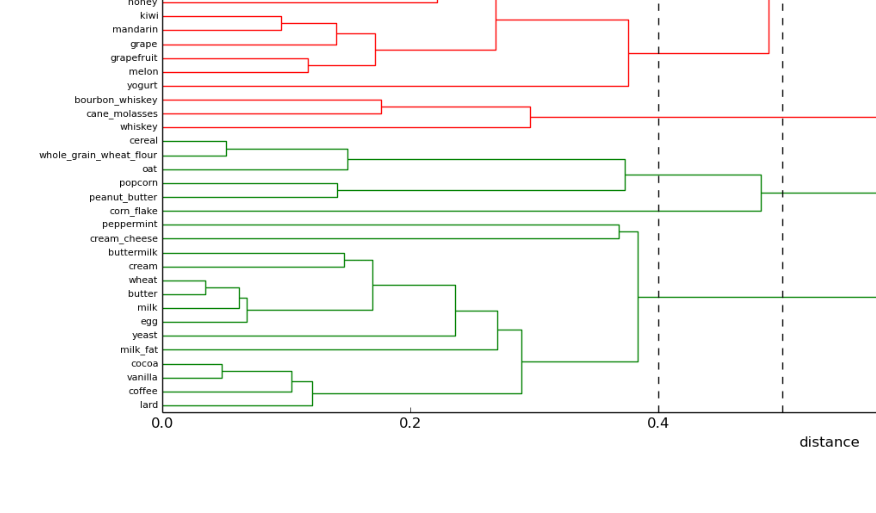
\includegraphics[width=3in]{dendrogram.png}
  \caption{The Dendrogram of Hierarchical Clustering Result}
  \label{fig:dendrogram}
\end{figure}

Procedures described above would select the vector file which best represents the ingredient data according to our similarity metric. And in the later part of the experiments, the selected vector file is used to calculate the contextual information of the ingredient with regard to the recipe.

\subsection{Optimization parameter settings}
\label{sec:Optimization parameter settings}
The realization of the optimization model exploits the contextual similarity metric that is discussed in \textbf{Section ~\ref{sec:Similarity Measures}} and the cosine similarity of the ingredient vectors.
For both similarity metrics, a context file is generated to describe the similarity scores between ingredients with the format on each line as:

\textit{ingredient\_name\_1, ingredient\_name\_2, similarity\_score}

According to the context file, a profit file is then generated to describe the profit each ingredient would bring to the recipe templates with format:

\textit{recipe\_index, ingredient\_name, profit\_score}

Furthermore, another profit file is generated to demonstrate the mean profit of each recipe with the format:


\textit{recipe\_index, mean\_profit\_score}

We choose to incorporate the contextual information with the co-occurrence information of ingredients for predicting the target ingredient. In the meantime, we also intend to discover the contribution of co-occurrence information in terms of making a correct prediction. Hence we design the configurations of experiments as listed below in Table ~\ref{table:exp settings}.


\begin{table}[!htb]
    \centering
    		\begin{tabular}{|p{1.8cm}|p{4.2cm}|}
			\hline
			Experiment No. & Configuration Settings \\ \hline
			1 & contexts with co-occurrence  \\ \hline
			2 & contexts only      \\ \hline
			3 & vector contexts with co-occurrence    \\ \hline
			4 & vector contexts only      \\ \hline
		\end{tabular}
	\caption{Experiment settings for different models}
    \label{table:exp settings}
\end{table}

The test data for this experiment, which contains 5,500 entries of recipes (10\% of total data set), is randomly sampled from original data set. For each recipe entry, a random ingredient is removed and then the rest of the ingredients form a recipe template as input to our model. According to the recipe template, the model suggests a list of possible ingredients to complete the recipe. In the ideal case, the removed ingredient would obtain the highest profit score and hence the smallest rank, which is rank one. Then some metrics listed in \textbf{Section ~\ref{sec:Evaluation Metrics}} will be calculated to evaluated the model performance of different configurations.

\section{Results}

In this section, results of the experiments discussed above are presented and discussed.

\subsection{Hyper-parameter Selection}

As illustrated in \textbf{Section ~\ref{sec:Word2Vec Parameter Settings}}, a range of values of different hyper-parameters are tried before model developing. Some critical parameters that we experimented on are $size$, $negative$, $cbow$ and $hs$. The results of training ingredient vectors with different hyper-parameter set can be seen below in Figure ~\ref{fig:hp-parameter}. The horizontal coordinate represents the range of parameters, while the vertical coordination denotes the average similarity scores among clusters.
In Figure ~\ref{fig:model}, the four configuration indicates the four combination of binary parameter $cbow$ and $hs$.

\begin{figure}[h!]
  \begin{subfigure}{1.5in}
    \centering
    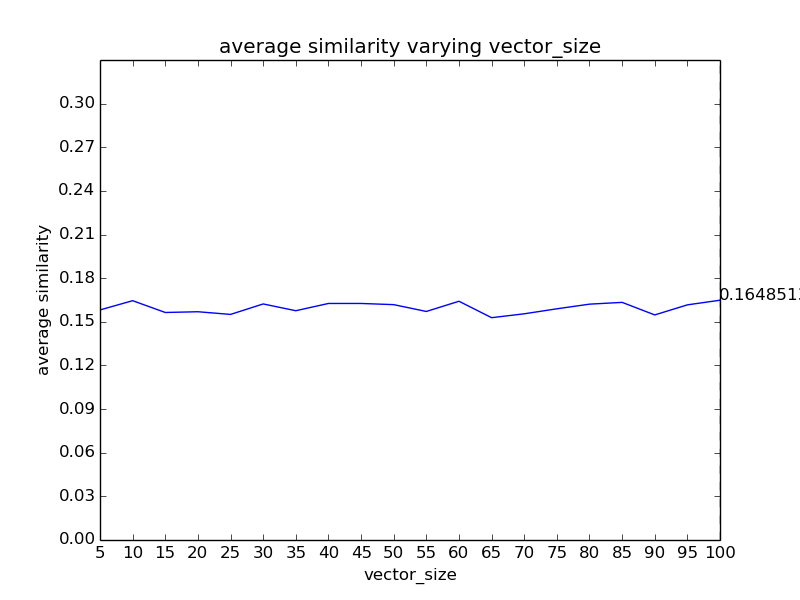
\includegraphics[width=\textwidth]{figure_compare_vector_size.png}
    \caption{Hyper-parameter : \newline size}
    \label{fig:size}
  \end{subfigure}%
  \begin{subfigure}{1.5in}
    \begin{subfigure}{\textwidth}
      \renewcommand\thesubfigure{\alph{subfigure}}
      \centering
      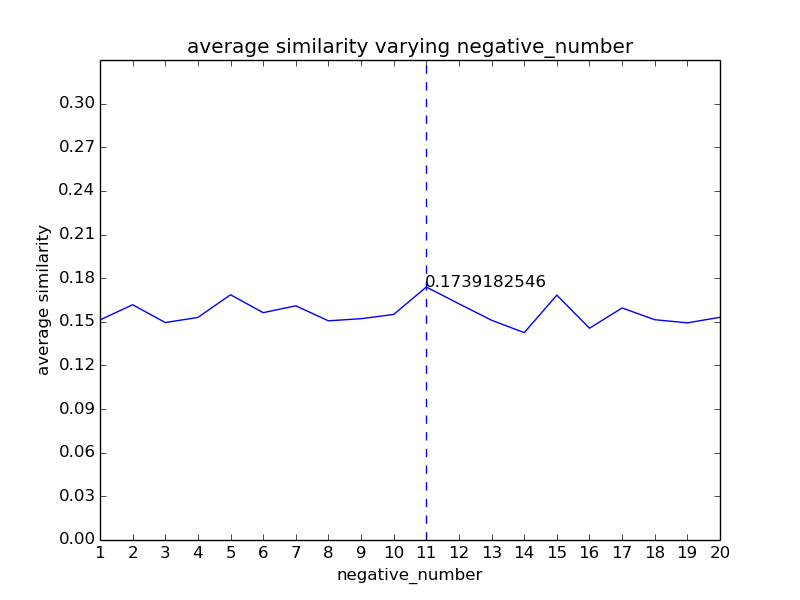
\includegraphics[width=\textwidth]{figure_compare_negative_number.png}
      \caption{Hyper-parameter : \newline negative number}
      \label{fig:negative}
    \end{subfigure}
    \begin{subfigure}{\textwidth}
      \renewcommand\thesubfigure{\alph{subfigure}}
      \centering
      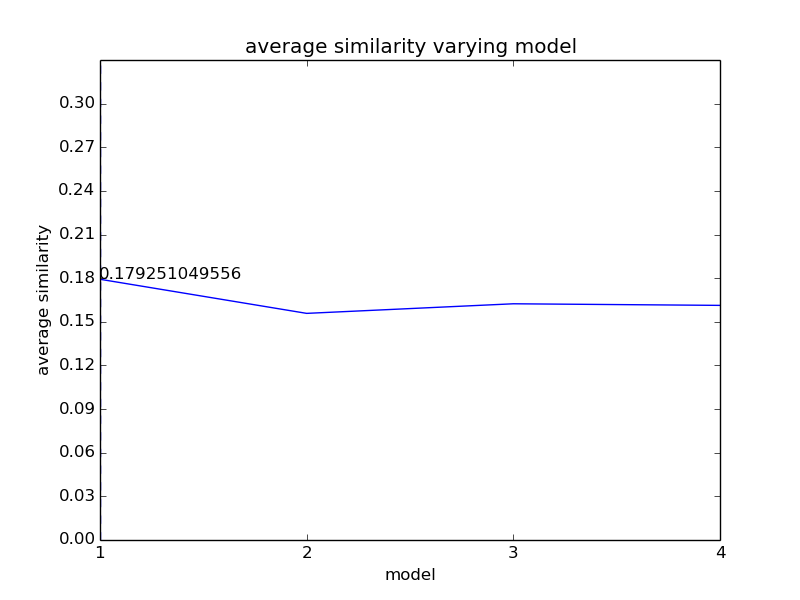
\includegraphics[width=\textwidth]{figure_compare_model.png}
      \caption{Hyper-parameter : \newline cbow \& hs}
      \label{fig:model}
    \end{subfigure}
    \label{fig:flat}
  \end{subfigure}
	\caption{Average Similarity variation according to different hyper-parameter settings}
	\label{fig:hp-parameter}
\end{figure}

As can be seen from the graphs, the best hyper-parameter settings are $size=100$, $negative\_number=11$, $cbow=0$ and $hs=0$. From this setting, the vector file is obtained.

\subsection{Similarity Metrics}

The contextual similarity of ingredients and the cosine similarity of ingredient vectors are calculated. As plotted in Figure ~\ref{fig:normalized_similarity_distribution} the distribution of normalized contextual similarity among 30,504 ingredient pairs, it is evident that the distribution is dense, mainly ranging from $0$ to $0.6$.

\begin{figure}[h!]
\centering
  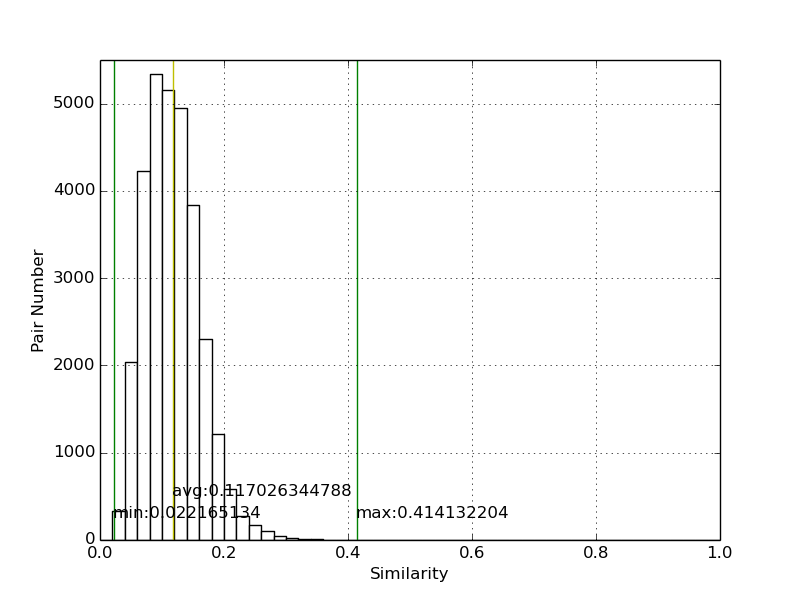
\includegraphics[width=2.5in]{normalized_similarity_distribution.png}
  \caption{The distribution of normalized contextual similarity scores among all ingredient pairs}
  \label{fig:normalized_similarity_distribution}
\end{figure}

And on the other hand, the distribution of angular similarity among ingredient vector pairs is demonstrated in Figure ~\ref{fig:angular_similarity_distribution}. As can be seen from the graph, the cosine similarity is also dense but within a different range -- $[0.4,1.0]$.

\begin{figure}[h!]
\centering
  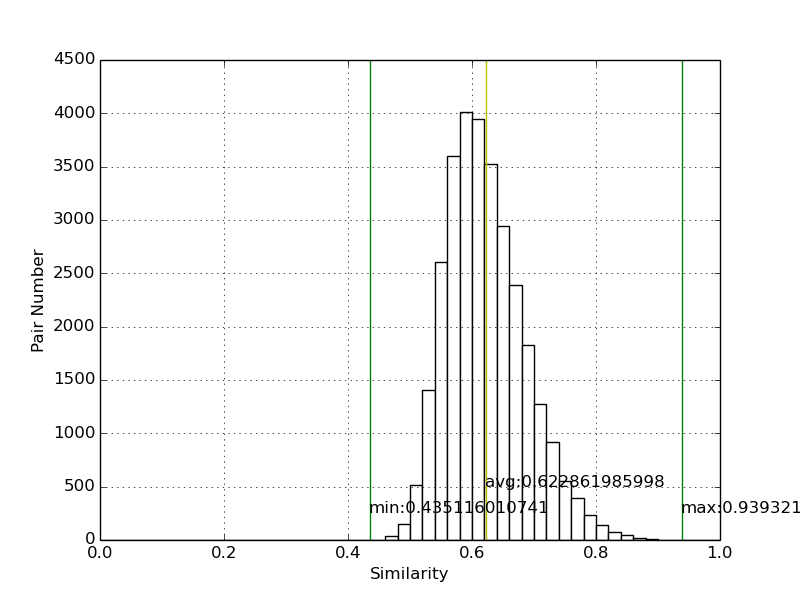
\includegraphics[width=2.5in]{angular_similarity_distribution.png}
  \caption{The distribution of angular similarity scores among all ingredient pairs}
  \label{fig:angular_similarity_distribution}
\end{figure}

It is worth mentioning that the normalized contextual similarity distribution centralized in small number (with average at 0.117). It may be due to the fact that it is common for different recipes to contain various combinations of ingredients. Hence in terms of an ingredient pair, their context is usually different, hence the generally low similarity score. While the distribution of the cosine similarity of ingredient vectors are different from that of contextual similarity, they share a similar shape dense shape of distribution.
Furthermore, as suggested in Figure ~\ref{fig:sim in category}, the average contextual similarity score in each food category is higher than the average among all ingredient pairs except for fruit and alcoholic beverage. It implies that the ingredients within the same food category may share similar context in a recipe.

\begin{figure}[h!]
\centering
  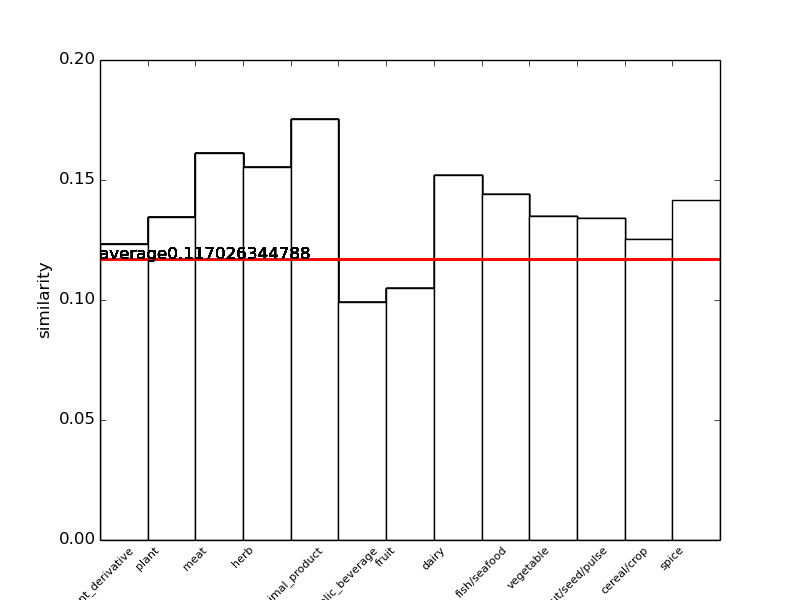
\includegraphics[width=2.5in]{normalized_similarity_by_category.png}
  \caption{The average similarity in each food category}
  \label{fig:sim in category}
\end{figure}

\subsection{Model Performance}


As introduced in \textbf{Section ~\ref{sec:Optimization parameter settings}}, some configurations of optimization model is tested to see the amount of contribution of contextual information and co-occurrence information to our prediction function.
And the result of experiment are shown below in Table ~\ref{table:model performance} with the best performance of each metric being highlighted in bold font.

\begin{table}[!htb]
    \centering
    	\begin{tabular}{|p{1.6cm}|p{1cm}|p{1cm}|p{1cm}|p{1cm}|}
	\hline

	Experiment No. & 1 & 2 & 3 & 4 \\ \hline
	Mean Rank & \textbf{24.6} & 39.6 & 32.7 & 62.2 \\ \hline
	Median Rank & \textbf{10.0} & 21.0 & 17.0 & 50.0 \\ \hline
	Rank$<=$10 (\%) & \textbf{51.9\%} & 33.0\% & 40.0\% & 10.0\% \\ \hline
	Rank=1 (\%) & \textbf{9.7\%}  & 3.4\% & 6.3\% & 1.0\% \\ \hline
	Mean AUC & \textbf{0.904} & 0.844 & 0.872 & 0.752 \\ \hline

	\end{tabular}
	\caption{Model performance with different configurations}
    \label{table:model performance}
\end{table}

From the results, it is clear that the best performance yields when using the contextual information with co-occurrence information. In general, using vector context information produces a worse result compared to using contextual information. Incorporating co-occurrence information improves the performance no matter which contexts file that we are using. Model with vector context information sees a even more drastic improvement in performance by taking the co-occurrence information into consideration. In terms of the mean and median rank in prediction of the missing ingredient, by taking co-occurrence information into consideration, the ranks are improved by more than 10 to the top. And the number of rank within 10 also increased nearly 20\%. And the correct prediction of the model also increased 6.3\%. In summary, both contextual information and co-occurrence information are important when making a prediction.

\section{Conclusions}

This paper proposed a model for suggesting ingredient to complete recipe template. Experiments are carried out for fine-tuning hyper-parameters while training ingredient vectors. Ingredients are compared with different similarity metrics. A carefully designed objective function is used for incorporating the contextual information and co-occurrence information of ingredients. Different model configurations are compared.
Results indicates that both contextual information and co-occurrence information contributes to the prediction.
A more comprehensive and flexible model for suggesting more than one ingredient for the recipe template or taking into consideration user's preferences will be part of the future work.

% include your own bib file like this:
%\bibliographystyle{acl}
%\bibliography{acl2015}

\begin{thebibliography}{9}

\bibitem[\protect\citename{Forbes et al.}2011]{Forbes:2011}
Forbes, P., and Zhu, M. 
\newblock 2011
\newblock Content-boosted matrix factorization for recommender systems: Experiments with recipe recommendation.
\newblock {\em Proceedings of Recommender Systems} (2011).

\bibitem[\protect\citename{Ueda et al.}2011]{Ueda:2011}
Ueda, M., Takahata, M., and Nakajima, S. 
\newblock 2011
\newblock User’s food preference extraction for personalized cooking recipe recommendation.
\newblock {\em Proc. of the Second Workshop on Semantic Personalized Information Management: Retrieval and Recommendation} (2011)

\bibitem[\protect\citename{Freyne et al.}2010]{Freyne:2010}
Freyne, J., and Berkovsky, S. 
\newblock 2010
\newblock Intelligent food planning: personalized recipe recommendation.
\newblock In {\em IUI,ACM} (2010), 321–324.

\bibitem[\protect\citename{Zhang et al.}2008]{Zhang:2008}
Zhang, Q., Hu, R., Mac Namee, B., and Delany, S.
\newblock 2008
\newblock Back to the future: Knowledge light case base cookery.
\newblock In {\em Proc. of The 9th European Conference on Case-Based Reasoning Workshop} (2008), 15.

\bibitem[\protect\citename{Wang et al.}2008]{Wang:2008}
Wang, L., Li, Q., Li, N., Dong, G., and Yang, Y.
\newblock 2008
\newblock Substructure similarity measurement in Chinese recipes. 
\newblock In {\em WWW, ACM} (2008), 979–988.

\bibitem[\protect\citename{Teng et al.}2012]{Teng:2012}
Chun-Yuen Teng , Yu-Ru Lin , Lada A. Adamic.
\newblock 2012
\newblock Recipe recommendation using ingredient networks.
\newblock In {\em Proceedings of the 3rd Annual ACM Web Science Conference}, p.298-307, June 22-24, 2012

\bibitem[\protect\citename{Clercq et al.}2016]{Clercq:2016}
Marlies De Clercq, Michiel Stock, Bernard De Baets, Willem Waegeman.
\newblock 2016
\newblock In {\em Data-driven recipe completion using machine learning methods}.
\newblock {\em Trends in Food Science \& Technology}, 49(2016) 1--13

\bibitem[\protect\citename{Ahn et al.}2011]{Ahn:2011}
Ahn, Y.\-Y., Ahnert, S. E., Bagrow, J. P., \& Barabasi, A. L. 
\newblock 2011
\newblock Flavor network and the principles of food pairing. 
\newblock In {\em Scientific Reports} 1.

\bibitem[\protect\citename{Mikolov et al.}2013]{Mikolov:2013}
Tomas Mikolov, Ilya Sutskever, Kai Chen, Greg S Corrado, and Jeff Dean.
\newblock 2013
\newblock In {\em Distributed representations of words and phrases and their compositionality}.
\newblock {\em Advances in Neural Information Processing Systems}, 26:3111--3119.




\end{thebibliography}

\end{document}
